Drinkkirobotti 5.0 on Pullonkaula ry:n, eli Tampereen yliopistossa toimivan tuotantotekniikan ammattiainekerhon opiskelijoiden vapaa-ajalla tekemä projekti. Robottisolu koostuu Yaskawan HC-10-monitoimirobotin "You Teach Me"\hyp{}solusta, ja sen ympärille rakennetuista baaritiskeistä. Drinkkirobottisolu näkyy kuvassa \ref{fig:drinkkirobotti}. You Teach Me on Yaskawan valmiiksi valmisteltu opetuskäyttöön tarkoitettu robottisolukokonaisuus \cite{Yaskawa2017}. Robottisolun  Baaritiskeissä on sisäpuolella pullohyllyt, ja kun robotilta tilataan juomaa, se hakee oikeat pullot hyllystä ja valmistaa niistä monikomponenttijuomia kaatamalla juomaa lasiin. Baaritiskin päällä on neljä mukipaikkaa, joihin robotti voi kaataa juomia.

\begin{figure}[h]
\begin{center}
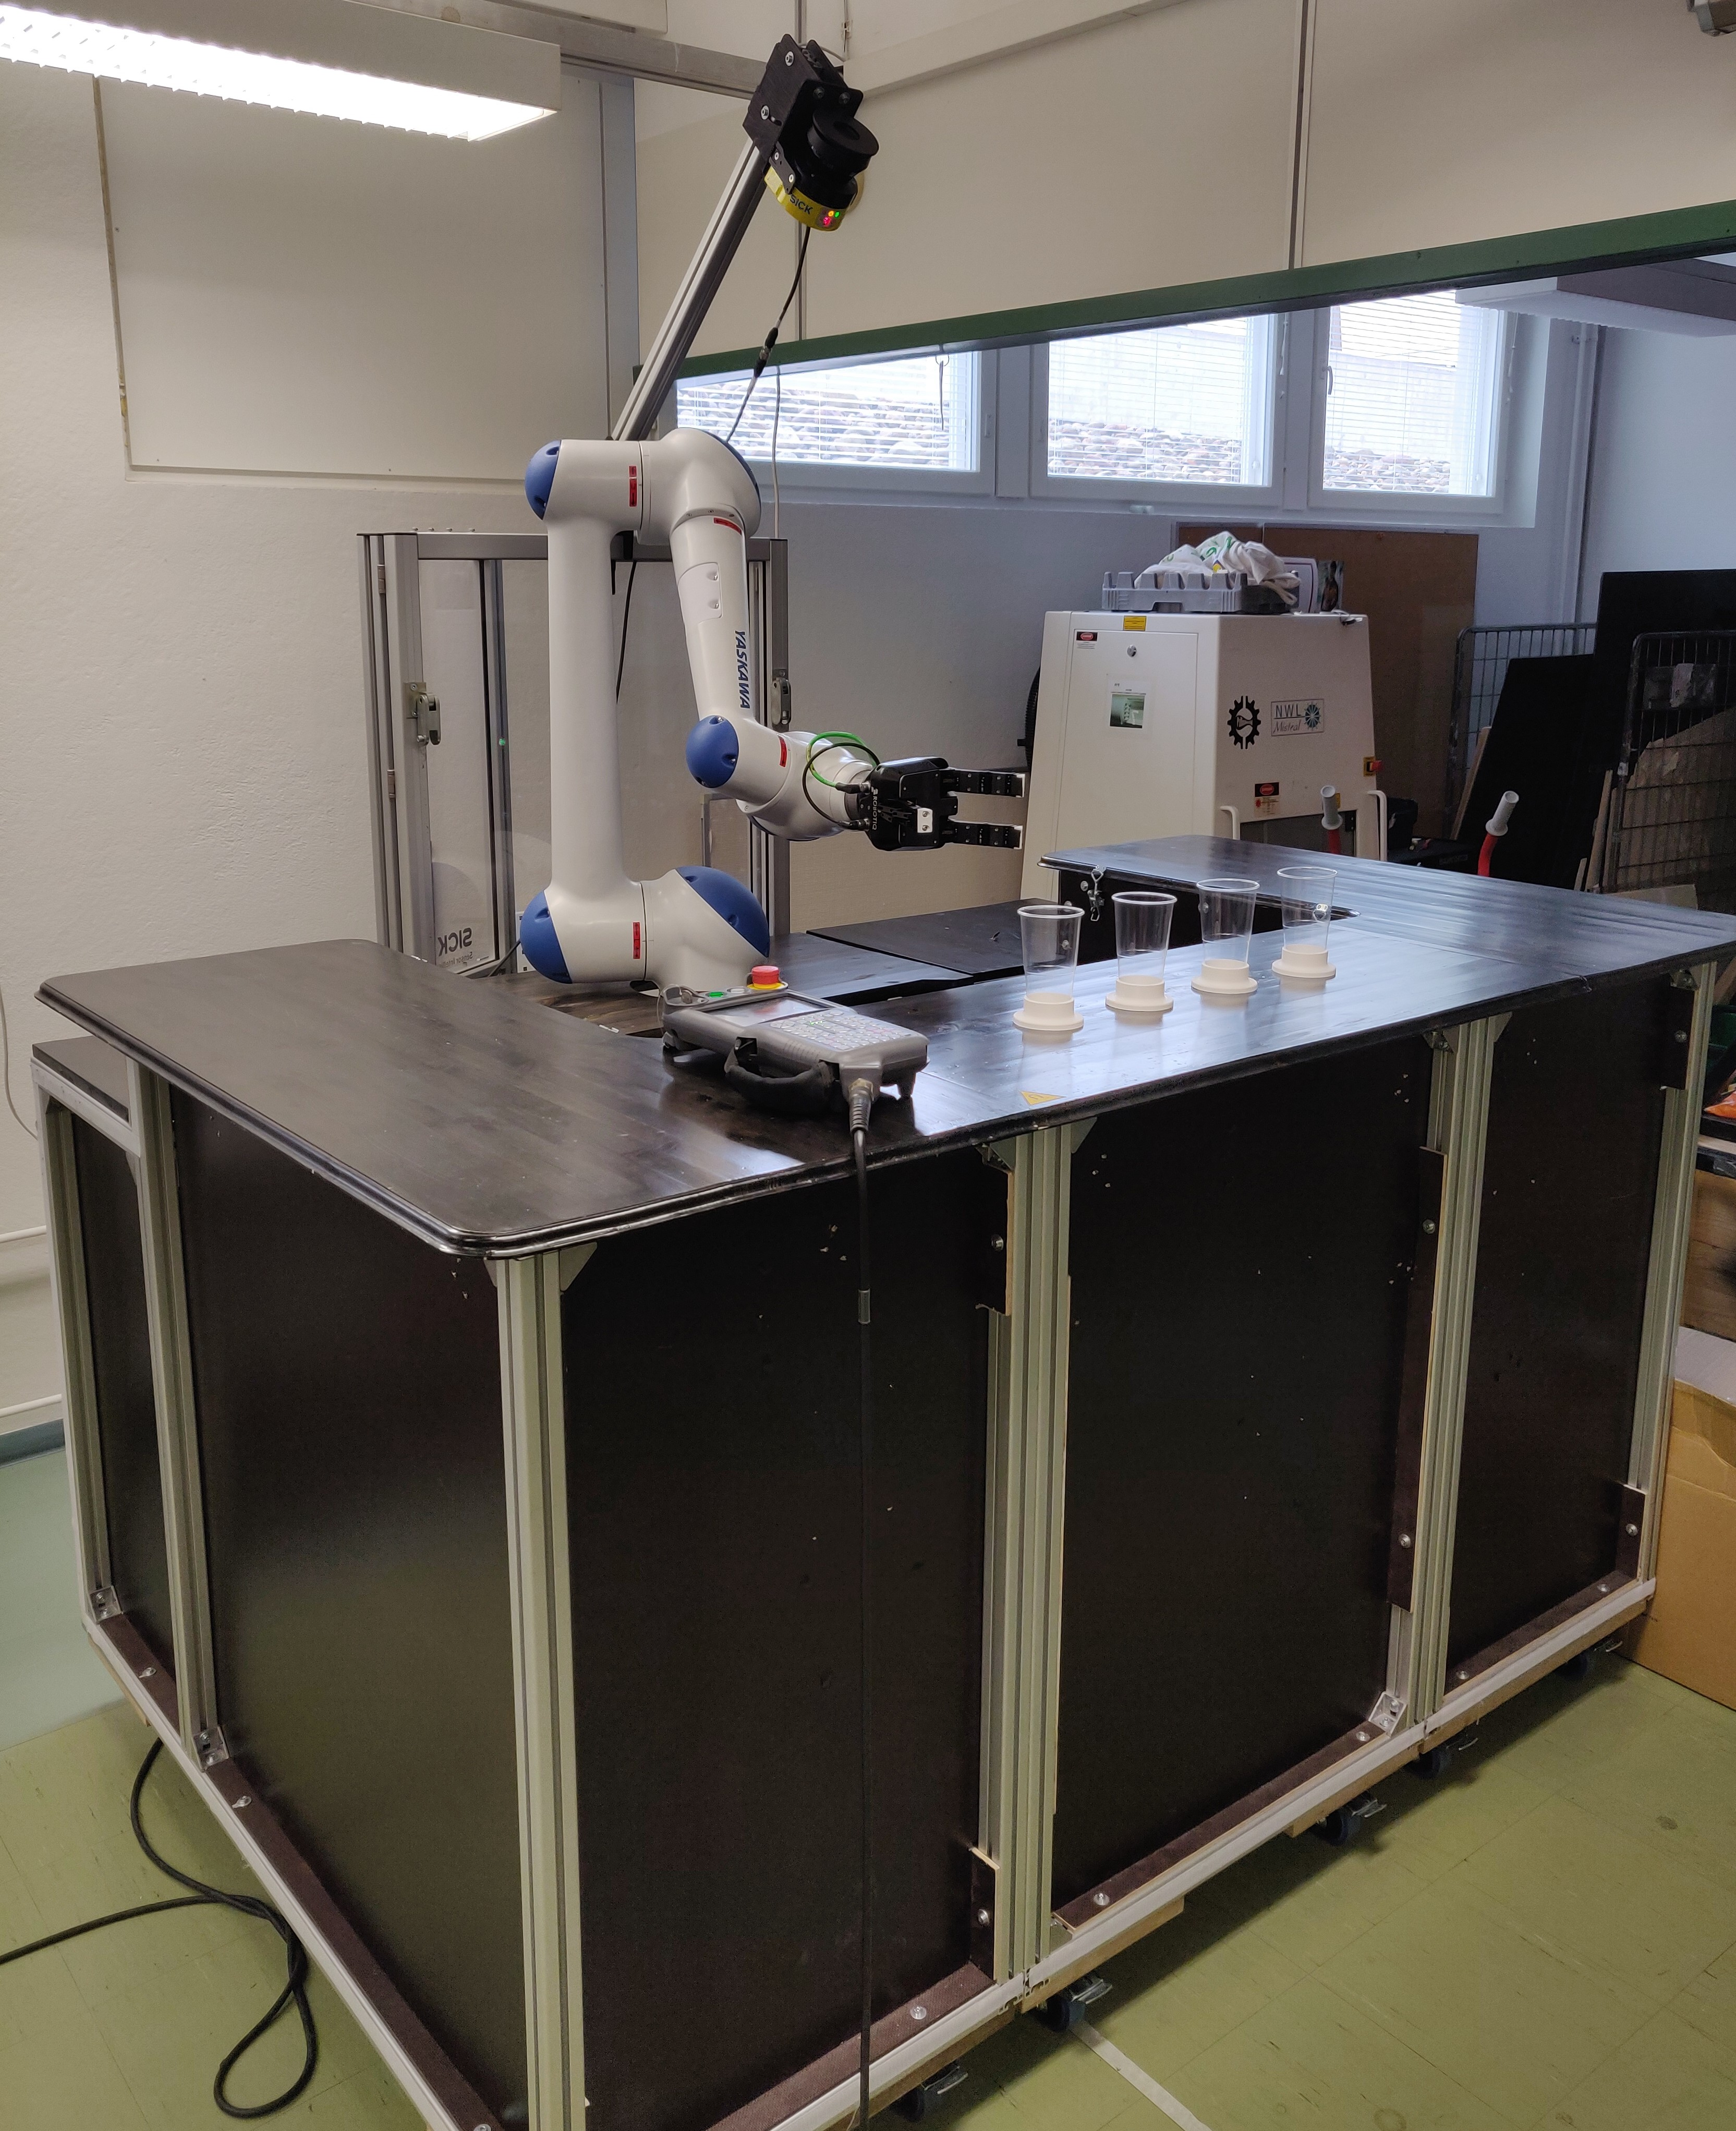
\includegraphics[scale=0.075]{img/drinkkirobotti.jpg}   % Scale 0.07 -> 0.075 -> Alla oleva teksti yhtä riviä alemmas.
\end{center}
\caption{Drinkkirobottisolu}
\label{fig:drinkkirobotti}
\end{figure}

\newpage

Robotilta juomien tilaaminen tapahtuu tabletille tehdyn käyttöliittymän avulla. Yaskawan HC-10 on yhteistyörobotti, eli se sisältää voima-antureita ja näiden avulla ihmisen ja robotin välinen yhteistyö on helpottunut. \cite{Pullonkaula2020}

\begin{figure}[h]
\begin{center}
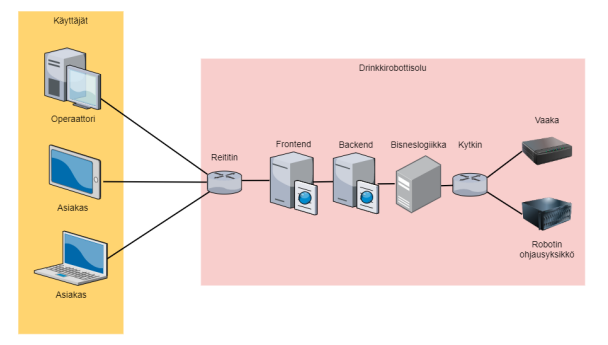
\includegraphics{img/rakenne_lowres.png}
\end{center}
\caption{Ohjelmistorakenne [lähde]}
\label{fig:rakenne}
\end{figure}

Drinkkirobotin ohjelmisto koostuu neljästä tasosta. Ohjelmistorakennetta on havainnollistettu kuvassa \ref{fig:rakenne}. Front end sisältää React.js:llä tehdyt käyttöliittymät operaattoria ja asiakasta varten. Operaattorinäkymästä voi esimerkiksi hallita robottisolun pullohyllyssä olevia pulloja lisäämällä tai poistamalla niitä ja valita robotin idle\hyp{}tilassa tekemiä liikkeitä. Asiakasnäkymästä voi selata tarjolla olevia juomia ja niiden sisältämiä komponentteja ja tilata juomia kerrallaan 1\hyp{}4 kappaletta. Back end toimii Node.js:llä ja se sisältää tiedon meneillään olevasta tapahtumasta missä juomia tarjoillaan ja siinä tapahtumassa tarjolla olevista juomista ja niiden komponenteista sekä määristä.

Itse robottikoodi on suhteellisen yksinkertaista. Siinä käytetään Yaskawan Inform \hyp{}ohjelmointikieltä, ja robottia ohjaa Yaskawan YRC-1000 -ohjausyksikkö. Robottikoodi sisältää "jobeja", jotka sisältävät robotin liikeratoja ja niiden parametrien määrittelyjä ja joissakin väleissä lyhyitä odotusaikoja. Robottisolun aivoina voidaan pitää sen bisneslogiikkatasoa, joka on kirjoitettu C\#-kielellä. Logiikka ohjaa robottia kertomalla, mikä funktio, eli "job" milloinkin suoritetaan. Se siis käsittelee front endiltä saadut tilaukset ja päättää esimerkiksi mikä pullo haetaan ja mihin lasiin juomaa kaadetaan. Logiikassa on myös reaaliaikainen tieto pullohyllyn tilanteesta, eli mitä pulloja hyllyssä on ja kuinka paljon juomaa missäkin pullossa on jäljellä. Kun operaattori lisää pullon, hän arvioi pullossa olevan juoman määrän ja merkitsee sen käyttöliittymään, jolloin juomamäärä välitetään logiikkaan. Kun pullosta kaadetaan juomaa, päivittyy uusi tieto pullossa olevasta juomasta. Jos pullossa on liian vähän juomaa jäljellä minkään drinkin tekoon, robotti poistaa pullon hyllystä automaattisesti. Näiden lisäksi robotin sisällä on Rasperry Pi-tietokone, joka ohjaa robotin tarttujaa. Tarttujaa voidaan ohjata robottikoodista siihen tarkoitetuilla jobeilla, jolloin robottikoodi kutsuu Rasperry Pi:tä.

Uusimpana lisäyksenä robottisoluun on implementoitu vaaka, joka on niin sanotulla pullonvaihtopisteellä. Vaa'an toiminta on hyvä esimerkki robotti-bisneslogiikkarajapinnasta, sillä vaa'an voi kalibroida ja sen kullakin hetkellä näyttämää arvoa voi kysyä logiikan avulla. Tämän vaa'an avulla robotti tunnistaa, onko pullonvaihtopisteellä pulloa. Tätä käytetään esimerkiksi uuden pullon lisäämisessä: Kun robotti hakee uutta pulloa hyllyyn, niin se pysähtyy ensin pullonvaihtopisteen eteen. Jos vaaka kertoo, että pullonvaihtopiste on tyhjä, logiikka ei käske robottia hakemaan olematonta pulloa, vaan käskee sen odottamaan tietyn ajan. Robotti hakee pullon vasta, kun se lisätään pullonvaihtopisteelle. Tämän toiminnallisuuden avulla robotti ei siis vie olematonta pulloa hyllyyn, jolloin back endissä olisi tieto pullosta tietyllä kohdalla pullohyllyä, vaikka pulloa ei oikeasti ole. Samoin, jos robotti on poistamassa pulloa pullohyllystä, ei se vie sitä pullonvaihtopisteelle jos siellä on jo pullo. Näin robotti ei työnnä vanhaa pulloa vaihtopisteeltä alas, vaan odottaa että se poistetaan sieltä. Työn alla on myös ominaisuus, jossa logiikka kertoo back endille, miten paljon juomaa lisätyssä pullossa on, ja operaattorin tehtäväksi jää vain tarkistaa lukema, eikä itse arvioida lisättävässä pullossa olevaa juoman määrää.
